\chapter{Sectionnement et Annotation d'entités}
\label{chap:structuration}

% court abstract
% Objectif: L'annotation manuelle peut atteirndre des interagréments raisonables (kappa) et nous démontrons qu'il est faisable d'automatiquement annoter les sections et métadonnées de référence d'un jugement à l'aide de modèle probabiliste graphiques comme le CRF ou le HMM moyennant de bien choisir les features
%Mots clés: annotation d'entités nommées judiciaires, chaine caché de markov, champ conditionnel aléatoires

\section{Introduction}
\label{sec:structuration:motivation}

\textcolor{red}{GENERALISER LE NOMBRE DE SECTION ET PRESENTER LES RESULTATS PUBLIES COMME ETANT UN CAS PARTICULIER}

Ce chapitre traite de la détection de sections et d'entités dans les décisions jurisprudentielles françaises. Ces décisions sont des documents non structurés qui partagent généralement la même structure qu'on peut définir par les sections: \textit{entête}, \textit{exposé du litige}, \textit{motifs}, \textit{dispositif}. Chaque section comprend des information sur l'affaire: 
\begin{enumerate}
\item la section ENTETE contient diverses métadonnées de référence (date, lieu, identifiant, parties impliquées, juges, affaires antérieurs liés, ...); 
\item La section CORPS qu'on peut diviser de manière plus fine pour distinguer:
\begin{itemize}
\item la section LITIGE comprend une description des faits, des procédures (jugements antérieurs, appel, assignations, ...), des demandes et raisonnements des parties; 
\item la section MOTIFS détaille le raisonnement et les arguments des juges;
\end{itemize}
\item la section DISPOSITIF est la décision finale qui résume la réponse des juges aux différentes demandes des parties.
\end{enumerate}

 Même si toutes les décisions respectent cette organisation, la structure à l'intérieur des sections peut varier d'un document à l'autre. Compte tenu de la répartition très sémantique des informations entre les sections, il nous a paru logique de détecter les sections dans un premier temps pour mieux organiser les différentes tâches d'extraction. Par la suite, des données sur les entités ou les demandes par exemple peuvent être plus facilement extraites en fonction des sections où elles se retrouvent généralement. Nous nous focalisons en particulier ici sur la détection d'entités telles que la date à laquelle le jugement a été prononcé, le type de juridiction, sa localisation (ville), les noms de juges, des parties et des avocats. La Table \ref{p4_relevantinfo} liste les différentes entités ciblées et fournit des exemples illustrant la forme de leurs mentions dans les arrêts français (décisions de juridictions de second degré).

\begin{table}[!ht]
\scriptsize
\begin{tabular}[c]{|p{0.17\textwidth}|c|p{0.37\textwidth}|cc|}
\hline
\textbf{Entités} & \textbf{Label} & \textbf{Exemples} & \multicolumn{2}{c|}{\textbf{\#mentions}$^a$}\\
  & & & \textbf{Médiane}$^b$& \textbf{Total}$^c$ \\ \hline
Numéro de registre & \textbf{rg} & "10/02324", "60/JAF/09" & 3 & 1318\\ \hline
Ville & \textbf{ville}& "NÎMES", "Agen", "Toulouse" & 3 & 1304\\ \hline
Juridiction & \textbf{juridiction} & "COUR D'APPEL" & 3 & 1308\\ \hline
Formation & \textbf{formation} & "1re chambre", "Chambre économique" & 2 &  1245\\ \hline
Date de prononcé de la décision & \textbf{date} & "01 MARS 2012", "15/04/2014" & 3 & 1590\\ \hline
Appelant & \textbf{appelant} & "SARL K.", "Syndicat ...", "Mme X ..." & 2 & 1336 \\ \hline
Intimé & \textbf{intime} & - // - & 3 & 1933 \\ \hline
Intervenant & \textbf{intervenant} & - // - & 0 & 51 \\ \hline
Avocat & \textbf{avocat} & "Me Dominique A., avocat au barreau de Papeete" & 3 & 2313\\ \hline
Juge & \textbf{juge} & "Monsieur André R.", "Mme BOUSQUEL" & 4 & 2089\\ \hline
Fonction de juge & \textbf{fonction} & "Conseiller", "Président" & 4 & 2062\\ \hline
Norme & \textbf{norme} & "l' article 700 NCPC", "articles 901 et 903" & 12 & 7641 \\ \hline
Argent & \textbf{argent} & "un euro", "" & 14$^*$ & 1777$^*$ \\ \hline
\noalign{\smallskip}\hline\noalign{\smallskip}
Non-entité & \textbf{O} & \textit{mot ne faisant partie d'aucune mention d'entité} & - & -\\ \hline
\end{tabular} 

$^a$ nombre de mentions d'entités dans le corpus annoté pour les expérimentations

$^b$ nombre médian de mentions par document dans le corpus annoté

$^c$ nombre total d'occurrences dans le corpus annoté

$^*$ Les statistiques sur les sommes d'argent ne concernent que 100 documents annotés (max=106, min=1, moyenne=17.77), contre 500 documents pour les autres entités.
\caption{Entités et labels correspondant utilisés pour labeliser leurs mots. }\label{p4_relevantinfo}
\end{table}


\section{Les décisions de justices françaises}
\label{sec:structuration:probleme}
\subsection{Structure}
Vu la sémantique ou le rôle des différentes sections, il est évident qu'elles sont séparées par des marqueurs bien précis. Une approche intuitive consiste par exemple à définir un algorithme capable de reconnaitre ces marqueurs de transitions à travers des expressions régulières. Cependant, les marqueurs utilisés ne sont pas standards car il n'existe pas de modèle stricte utilisé par toutes les juridictions. par conséquent, les marqueurs de transitions sont souvent différents d'une décision à l'autre et peuvent être des titres ou des motifs à base de symboles (astérisques, tirets, etc.). Il arrive parfois que la transition soit implicite et qu'on ne s'en rende compte que par la forme des lignes, au cours de la lecture. Même les marqueurs explicites sont hétérogènes. D'une part en cas d'utilisation de titres par exemple, la transition de l'entête à l'exposé du litige peut être indiquée par des titres comme "\textit{Exposé}", "\textit{FAITS ET PROCÉDURES}", "\textit{Exposé de l’affaire}", "\textit{Exposé des faits}", etc. Quant au dispositif, il est introduit généralement par l'expression "\textit{PAR CES MOTIFS}" avec souvent quelques variantes qui peuvent être très simples (par ex. "\textit{Par Ces Motifs}") ou exceptionnelles (par ex. "\textit{P A R C E S M O T I F S :}"). Dans certaines décisions, cet expression est remplacée par d'autres expressions comme "\textit{DECISION}", "\textit{DISPOSITIF}", "\textit{LA COUR}", etc. 
D'autre part lors de l'utilisation de symboles, il arrive qu'un même motif sépare différentes sections et même des paragraphes dans le même document.

Une hétérogénéité similaire apparait pour les entités. Les noms de parties et d'avocats sont généralement placés après un mot particulier comme  "\textit{APPELANTS}" ou "\textit{DEMANDEUR}" pour les demandeurs (appelants en juridiction de 2e degré), "\textit{INTIMES}" ou "\textit{DEFENDEUR}" pour les défendeurs (ou intimés), and "\textit{INTERVENANTS}" pour les intervenants. Les noms des individus, sociétés et lieux commencent par une lettre majuscule ou sont entièrement en majuscule. Cependant, certains mots communs peuvent apparaitre aussi en majuscule (par ex. \textit{APPELANTS}, \textit{DÉBATS}, \textit{ORDONNANCE DE CLÔTURE}). Les entités peuvent contenir des chiffres (identifiant, dates, ...), des caractères spéciaux ("/", "-"), des initiaux ou abréviations.  Dans l'entête, les entités apparaissent généralement dans le même ordre (par ex. les appelants avant les intimés, les intimés avant les intervenants). Cependant, plusieurs types d'entités apparaissent dans l'entête, contrairement aux autres sections où seules les normes nous intéressent dans cette étude. L'entête est aussi mieux structurée que les autres sections même si sa structure peut différer entre deux documents.

\subsection{Acquisition}
Les décisions sont disponibles auprès des juridictions mais on note qu'un certain nombre d'entre elles est accessible en ligne. On les y retrouve sous divers formats dont par exemple .rtf sur \url{http://legifrance.gouv.fr}, ou .doc(x) et .txt sur le site web de LexisNexis d'où proviennent les documents de notre étude. Chaque document téléchargé de LexisNexis contient une ou plusieurs décisions de justice. De plus, LexisNexis n'autorise le téléchargement simultané qu'un nombre très faible de décisions qui décroit dans le temps (nous avons remarqué des limites de 100, puis 20, et ensuite 10 au cours de ces 3 dernières années). Par contre, l'identification et le service des documents sur Legifrance permet de pouvoir récolter plus rapidement les documents à l'aide par ex. d'une simple routine de téléchargement itératif.




\section{Reconnaissance d'entités par étiquetage de séquence}
\label{sec:structuration:biblio}

\subsection{Approches générales de détection d'entités}

Quatre catégories d'approches de détection d'entités ont été distinguées \citep{chau2002nerwithNN}:

\begin{itemize}
\item Les \textbf{systèmes à recherche lexicale} sont conçus sur la base d'une liste d'entités précédemment connues, avec leurs synonymes dans le domaine d'intérêt. Par exemple, dans le domaine juridique, un lexique pourrait contenir les identifiant de règles juridiques et les noms des juges. La liste des entités peut être manuscrite par des experts ou apprise à partir d'un ensemble de données étiquetées (phase d'apprentissage). Cependant, il s'avère très difficile de maintenir une telle liste car le domaine pourrait changer régulièrement (nouvelles lois par ex.). De plus, les mentions d'entités peuvent avoir plusieurs variantes. Par exemple, la même règle "Article 700 du code de procédure civile" peut \^etre citée seule et en entier (\textit{article 700 du code de procédure civile}), ou abrégée (\textit{article 700 CPC}), ou encore combinée avec d'autres règles (\textit{articles 700 et 699 du code de procédure civile}). Ces problèmes, y compris les ambiguïtés (par exemple, différentes entités utilisant les mêmes mots), ont limité les premiers systèmes \citep{palmer1997learnedLookup}.

\item Les \textbf{systèmes à base de règles} décrivent suffisamment la diversité des mentions d'entités en fonction de la régularité du contexte, de la structure et du lexique. Ils sont avantageux parce que leurs erreurs sont facilement explicables. La définition manuelle de règles exige malheureusement des efforts considérables, en particulier pour les grands corpus. De plus, un ensemble donné de règles est difficilement réutilisable dans d'autres domaines. Cependant, quelques approches adaptatives ont été conçues pour surmonter ces limites tout en bénéficiant toujours de facilité à expliquer le comportement des systèmes à base de règles \citep{siniakov2008gropusrulebased,chiticariu2010adaptativerulebased}.

\item Les \textbf{systèmes statistiques} adaptent les modèles statistiques de langage, issus typiquement des méthodes de compression de texte, pour détecter les entités. Par exemple, \citet{witten1999languagemodel} ont adapté les schémas de compression nommés "Prédiction par Correspondance Partielle".

\item Les \textbf{systèmes basés sur l'apprentissage automatique} exécutent des classifieurs multi-classes sur des segments de texte. Par exemple, un classifieur traditionnel comme le classifieur bayésien naïf peut être entrainer pour détecter les noms de gènes en classifiant les mots du documents à partir d'un ensemble de descripteurs définis manuellement \citep{persson2012nbbioner}. Pour détecter les entités, les algorithmes d'étiquetage de séquence tels que le CRF quant à eux classifient les segments de texte tout en modélisant les transitions entre les labels \citep{finkel2005stanfordcrfner}. Dans ce registre, les architectures d'apprentissage profond réalisent actuellement les meilleures performances sur de multiples tâche d'extraction d'information en général et de reconnaissance d'entités nommées en particulier \citep{lample2016nnner}.
\end{itemize}
Certains travaux ont combiné diverses approches pour extraire les entités à partir de documents juridiques,  par exemple,  par la description de l'information contextuelle en utilisant des règles pour répondre au problème d'ambigüité des méthodes à recherche lexicale \citep{mikheev1999NERlexicalWithRules,hanisch2005prominer}. 

\subsection{Détection d'entités dans des documents juridiques}

Les modèles HMM et CRF ont été utilisés dans de multiples travaux pour reconnaître des entités juridiques. Ils peuvent être combinés à d'autres approches dans un système global. Après avoir segmenter les documents à l'aide d'un modèle CRF, \citet{dozier2010legalnerr} ont combiné plusieurs approches pour reconnaître des entités dans les décisions de la cour suprême des Etats-Unis. Ils ont définis des détecteurs distincts à base de règles pour identifier séparémment la juridiction (zone géographique), le type de document, et les noms des juges, en plus de l'introduction d'une recherche lexicale pour détecter la cour, ainsi qu'un classifieur entrainé pour reconnaître le titre. Ces différents détecteurs ont atteint des performances prometteuses, mais avec des rappels limités entre $ 72 \% $ et $ 87 \% $. Suivant la complexité des éléments à extraire, un système peut comprendre des indexes lexicaux pour les motifs simples et non-systématiques (indicateurs de résultats ou de parties) et les règles pour des motifs plus complexes et systématiques (par ex. noms de juges, énoncés de décisions) \citep{Waltl2016lexia, wyner2010extractlegalelts}. \citep{cardellino2017legalNERCL} quant à eux ont utilisé le CRF et les réseaux de neurones (\textcolor{red}{OÙ pays?}). Les basses performances qu'ils rapportent pour l'extraction dans les jugements illustre bien la difficulté de la détection d'entités juridiques. Plus récemment encore, \citet{andrew2018legalNerAndRelation} obtiennent de bons résultats en combinant l'extraction d'entités non-juridiques par CRF à l'extraction de relations par une grammaire GATE JAPE \citep{thakker2009gatejape} sur des décisions du Luxembourg rédigées en français.

La comparaison avec d'autres approches démontre bien que les modèles probabilistes atteignent de très bonnes performances lors de l'extraction d'information dand les documents juridiques. Par exemple, le HMM a été comparé à l'Algorithme de Perceptron à Marges Inégales (PAUM) \citep{li2002PAUM} pour reconnaître les institutions et références d'autres décisions de justice, ainsi que les citations d'actes juridiques (loi, contrat, etc.) dans les décisions judiciaires de la République Tchèque \citep{Kriz2014nerinczechdecisions}. Les deux modèles ont données de bonnes performances avec des scores F1 de $ 89 \% $ et $ 97 \% $ pour le HMM utilisant les trigrammes comme descripteurs de mots, et des scores F1 de $ 87 \% $ et $ 97 \% $ pour le PAUM en utilisant des 5-grammes de lemmes et les rôles grammaticaux (\textit{Part-Of-Speech tag}) comme descripteurs. 

\subsection{Modèles d'étiquetage de texte}

Considérons un texte T comme étant une séquence d'observations $t_{1:n}$, avec chaque $t_i$ étant un segment de texte (mots, ligne, phrase, etc.). En considérant une collection de labels, l'étiquetage de T consiste à affecter à les labels appropriés à chaque $t_i$. La segmentation de T est un étiquetage particulier qui implique de découper T en des groupes qui ne se chevauchent pas (des partitions), tels que les segments d'un groupe constituent nécessairement une sous-séquence de T. En d'autres termes, segmenter T revient à labeliser ses segments en considérant une contrainte particulière (\textcolor{red}{Laquelle?}). Parmi les multiples modèles d'étiquetage de séquences, nous nous sommes proposés d'étudier les performances de quelques modèles établis décrits ci-après.
\subsubsection{HMM}
Un modèle HMM est une machine à état fini défini par un ensemble d'états $ \lbrace s_1, s_2, ..., s_m \rbrace $. Un modèle HMM a pour fonction d'affecter une probabilité jointe 
$ P (T , L) = \prod\limits_i P(l_i \vert l_{i-1})P(T \vert l_i)$  à des paires de séquences d'observations $ T = t_{1: n} $ et de séquence de labels $ L = l_{1:n} $. Etant donnée qu'un HMM est un modèle génératif, chaque label $l_i$ correspond à l'état $s_j$ dans lequel la machine a généré l'observation $t_i$. Il y a autant de labels possibles que d'états. Le processus de labelisation de T consiste à déterminer la séquence de labels $ L^* $ qui maximise la probabilité jointe ($L^* = \arg \max\limits_L P(T, L)$). Une évaluation de toutes les séquences possibles de labels est nécessaire pour déterminer celle qui convient mieux à $ T $. Pour éviter la complexité exponentielle $ O(m^n)$ d'une telle approche, $n$ étant la longueur de la séquence et $m$ le nombre de labels possibles, le processus d'étiquetage utilise généralement l'algorithme de décodage Viterbi \citep{viterbi1967viterbi} qui est basé sur la programmation dynamique. Cette algorithme utilise les paramètres du HMM estimés par apprentissage sur un corpus de textes annotés manuellement:
\begin{itemize}
\item Un ensemble d'états $ \lbrace s_1, s_2, ..., s_m \rbrace $ et un alphabet $ \lbrace o_1, o_2, ..., o_k \rbrace $
\item La probabilité que $ s_j $ génère la première observation $ \pi(s_j), \forall j \in [1 .. m] $
\item La distribution de probabilité de transition $ P (s_i\vert s_j),  \forall i,j \in [1 .. m] $
\item La distribution de probabilité de d'émission $ P(o_i\vert s_j), \forall i \in [1 .. k], \forall j \in [1 .. m]$
\end{itemize}

Les probabilités de transition et d'émission peuvent être inférer en utilisant une méthode de maximum de vraisemblance comme l'algorithme d'espérance maximale. L'algorithme Baum-Welch \citep{welch2003baumwelch} en est une spécification conçu spécialement pour le HMM. L'avantage du HMM réside dans sa simplicité et sa vitesse d'entrainement. Par ailleurs, il est difficile de représenter de multiples descripteurs interactifs pour les segments de texte, tout comme de modéliser la dépendance entre des observations distantes parce que l'hypothèse d'indépendance entre observations est très restrictive (i.e. l'état courant dépend uniquement des état précédents et de l'observation courante). \citet{rabiner1989tutorial} fournit plus de détails sur le HMM.

\subsubsection{CRF}
\label{sec:structuration:biblio:CRF}

Même si l'algorithme Viterbi est aussi utilisé pour appliquer le CRF à l'étiquetage de séquence, les structures du CRF et du HMM diffèrent. Au lieu de maximiser la probabilité jointe $ P(L, T)$ comme le HMM, un CRF \citep{lafferty2001crfie} cherche la séquence de labels $L^*$ qui maximise la probabilité conditionnelle suivante: $$P(L|T) = \frac{1}{Z}\exp \left(\sum\limits_{i=1}^n\sum\limits_{j=1}^F \lambda_j f_j(l_{i-1},l_i,t_{1:n},i)\right)$$ où $Z$ est le facteur de normalisation. Les fonctions potentielles $f(\cdot)$ sont les caractéristiques utilisés par les modèles CRF. Deux types de fonctions caractéristiques sont définies: les caractéristiques de transition qui dépendent des labels aux positions courantes et précédentes ($l_{i-1}$ and $ l_{i}$ respectivement) et de $T$; et les caractéristiques d'état qui sont des fonctions de l'état courant $ l_{i} $ et de la séquence $ T $. Ces fonctions $f(\cdot)$ sont définies à l'aide soit par de fonctions à valeur binaire ou réelle $b(T,i)$ qui combine les descripteurs d'une positiond'une position $i$ dans $T$ \citep{Wallach2004crfintro}. Pour labéliser les références aux règles de loi par exemple, un CRF pourrait inclure par exemple les fonctions potentielles pour labéliser "\textit{700}" dans ce contexte "\textit{... l'article 700 du code de procédure civile...}":
{\scriptsize
\[f_1(l_{i-1},l_i,t_{1:n},i) = \left\lbrace \begin{array}{ll}
b_1(T,i) & \text{si } l_{i-1} = \text{NORME} \wedge l_i = \text{NORME} \\
0 & \text{otherwise}
\end{array} \right.\]
\[f_2(l_{i-1},l_i,t_{1:n},i) = \left\lbrace \begin{array}{ll}
b_2(T,i) & \text{si }l_i = \text{NORME} \\
0 & \text{otherwise}
\end{array} \right.\]
avec
\[b_1(T,i) = \left\lbrace \begin{array}{ll}
1 & \text{si } (t_{i-1} =\text{article) }\wedge (POS_{i-1}=\text{NOM}) \\&  \wedge  (NP1_{i-1}=\text{<unknown>)} \wedge (NS1_{i-1}=\text{@card@)} \\
0 & \text{otherwise} 
\end{array} \right.\]
\[b_2(T,i) = \left\lbrace \begin{array}{ll}
1 & \text{si } (t_i =\text{700) }\wedge (POS_i=\text{NUM})  \wedge (NP1_i=\text{article)} 
\wedge (NS1_i=\text{code)} \\
0 & \text{otherwise}
\end{array} \right.\]
}
$t_i$ étant une observation dans $T$, POS étant le rôle grammatical de $t_i$ (NUM = valeur numerique, NOM=nom), et NP1 et NS1 sont les lemmes des mots avant et après $t_i$, respectivement. Les symboles \textit{<unknown>} et \textit{@card@} encode les lemmes inconnus et les lemmes de numbres respectivement. Pouvant être activées au même moment, les fonctions $f_1$ et $f_2$ définissent des descripteurs se chevauchant. Avec plusieurs fonctions activées, la croyance dans le fait que $l_i = NORME$ est renforcée par la somme $\lambda_1 + \lambda_2$ des poids  des functions activées \citep{Zhu2010CRFlecture}.  Un modèle CRF emploie une fonction $f_j$ lorsuqe ses conditions sont satisfaites et $\lambda_j > 0$. Les diverse fonctions pondérées $f_j$ sont définies par des descripteurs caractérisant le texte et les labels des données d'entrainement. La phase d'entrainement consiste principalement à estimer le vecteur de paramètres $\lambda = (\lambda_1,...,\lambda_F)$ à partir des de textes annotés manuellement $ \lbrace (T_1, L_1), ..., (T_M, L_M) \rbrace $, $ T_k $ étant un texte et $ L_k $ la séquence de labels correspondande. La valeur optimal retenue pour estimer de $\lambda$ est celle maximisant la fonction objectif   
$\sum\limits_ {k = 1} ^ M \log P (L_k \vert T_k) $ sur les données d'entrainement. En général, outre le maximum de vraisemblance, cette optimisation est résolue à l'aide de l'algorithme de descente du gradient dont l'exécution peut-être accélérée à l'aide de l'algorithme L-BFGS \citep{liu1989l-bfgs}.

\subsubsection{Extensions neuronales du CRF}
2015 https://arxiv.org/pdf/1508.01991.pdf

https://github.com/UKPLab/emnlp2017-bilstm-cnn-crf

dnn crf : https://pdfs.semanticscholar.org/c322/7702dd212965157a615332f3dd78b0f11b5e.pdf

https://towardsdatascience.com/conditional-random-field-tutorial-in-pytorch-ca0d04499463

Deux architectures de réseaux de neuronnes réalisent actuellement les meilleures performances en matière de détection d'entités nommées. Il s'agit du modèle LSTM-CRF proposé par \citet{lample2016nnner} et du LSTM-CNN-CRF de \citet{ma2016lstm-cnns-crf}. On pourrait résumer ces architectures en trois phases. Dans un premier temps, les segments de textes (mots) sont représentés vectoriellement en concatenant 2 vecteurs de plongement sémantique: l'un issu de l'apprentissage morphologique du mot à partir de ces caractères, et l'autre issu de l'apprentissage du contexte général d'occurrence du mot (par ex. CBOW, Skip-gram, Glove, ...). Lors de la seconde phase, deux couches de cellules LSTM enchainées permettent de modéliser le contexte à droite et à gauche de chaque mots du texte. La dernière phase détermine la séquence de label la plus probable pour le texte à l'aide d'une implémentation d'un modèle CRF sous forme de réseau de neuronnes. Le CRF reçoit en entrée la concaténation des contextes à droite et à gauche des mots.

\subsection{Définition des descripteurs d'éléments atomiques}
\textcolor{red}{Pourquoi? Quoi ? et Comment?}

La représentation des éléments atomiques occupe une place importante dans le bon fonctionnement des modèles décrits précédemment. Si les architectures basée sur les LSTM combinent une représentation indépendente de la tâche à des représentations de forme et de contexte inférerées en interne, la définition des descripteurs est plus arbitraire chez les modèles probabilistes. Il s'agit généralement de caractéristiques booléennes comme celles mentionnées dans la description du CRF (\ref{sec:structuration:biblio:CRF}). Par exemple, indiquer si un mot débute par une lettre majuscule permet de mettre en évidence les noms propres. La définition de telles caractéristiques consiste ainsi à fournir au modèle des indices l'aidant à mieux distinguer les différents types d'entités par la forme et le contexte d'occurrence des éléments atomiques. 

Etant donné que les descripteurs dépendent généralement de l'intuition du modélisateur, il est difficile mais nécessaire d'identifier des descripteurs appropriés. Les nombreux travaux de reconnaissance d'entités nommés inspirent des descripteurs candidats qui ont déjà été expérimentés avec succès. De plus, il est possible d'appliquer une sélection des descripteurs afin de réduire tous les candidats définis à un sous-ensemble plus optimal. Cette réduction a pour objectif d'améliorer les performances d'étiquetage, d'accélérer les phases d'extraction de caractéristiques, d'entrainement et de prédiction, et de fournir une meilleure compréhension du comportement des modèles. 

Les méthodes de sélection utilisées dans la littérature sont généralement basées sur des algorithmes Filtre (\textit{filters}) qui associent à chaque descripteur un score, ou des algorithmes Symbiose (\textit{wrappers}) qui préparent, évaluent et comparent des combinaisons de descripteurs. D'une part, les filtres ont l'avantage d'être rapide à exécuter par rapport aux emballages beaucoup plus lents. D'autre part, les filtres sont moins performants car ils ne permettent pas d'éviter les cas de redondances et ne prennent pas en compte l'effet de la combinaison de variables. C'est ainsi que les filtres peuvent être utilisés avant les emballages afin de comparer uniquement les combinaisons des caractéristiques significatives. Au départ proposés et utilisés en classification multi-dimmensionnelle, les algorithmes de sélections de caractéristiques ont été appliqués avec succès pour l'extraction d'entités. \citet{klinger2009FeaturefilterCRF} ont 

\subsection{Sélection du schéma d'étiquetage}
Nous traitons d'entités dont les mentions comprennent un ou plusieurs éléments atomiques. Pour améliorer les performance d'un modèle d'étiquetage, certaines parties des entités peuvent être mise en évidence à travers une représentation appropriée de segment. Nous comparons dans cette étude quelques schémas d'étiquetage dont certains sont décrits par \citet{konkol2015tagModel}. Le schéma IO utilisé par défaut ne met l'accent sur aucune partie de l'entité et affecte le même label à chaque élément de l'entité. D'autres schémas distinguent soit le premier élément (BIO), soit le dernier (IEO), soit les deux (BIEO). Les schémas IEO2 BIO2 sont des variantes respectives des schémas IEO et BIO. Elles utilisent resp. les préfixes E- et B- pour étiqueter les entités à mot unique, contrairement à IEO1 et BIO1 qui utilisent plutôt le préfixe I-. Le modèle BIEO est souvent étendu à BIESO (ou BILOU) dans le cas où on souhaite distinguer les mentions à un seul élément (par ex. ville ou numéro RG). Les lettres des sigles de ces modèles servent de préfixes aux labels et portent la signification suivante:

\begin{itemize}
\item B - "\textit{beginning}": début;
\item I - "\textit{inside}": intérieur;
\item E (ou L, ou M) - "\textit{end}" ou "\textit{last}" ou "\textit{middle}": fin;
\item S (ou U, ou W) - "\textit{single}" ou "\textit{unit}" ou "\textit{whole}": singleton;
\item O - "\textit{outside}": hors de toute entité.
\end{itemize}

La figure \ref{p4_sample-tagmod} illustrate l'utilisation des ces différents modèles sur un extrait de décision de justice:
\begin{figure}[!h]
\tiny
\begin{tabular}{l|ccccccccccc}
 & \textit{composée} & \textit{de} & \textit{Madame} & \textit{Martine} & \textit{JEAN} & , & \textit{Président} & \textit{de} & \textit{chambre} & , & \textit{de} \\ 
IO & O & O & I-JUGE & I-JUGE & I-JUGE & O & I-FONCTION & I-FONCTION & I-FONCTION & O & O \\
BIO & O & O & B-JUGE & I-JUGE & I-JUGE & O & B-FONCTION & I-FONCTION & I-FONCTION & O & O \\
IEO & O & O & I-JUGE & I-JUGE & E-JUGE & O & I-FONCTION & I-FONCTION & E-FONCTION & O & O \\
BIEO & O & O & B-JUGE & I-JUGE & E-JUGE & O & B-FONCTION & I-FONCTION & E-FONCTION & O & O \\
\end{tabular}
\caption{Illustration de différents schémas d'étiquetage}\label{p4_sample-tagmod}
\end{figure}

Il est possible d'aller plus loin en mettant l'accent sur les mots avant  (O-JUGE) et après (JUGE-O) l'entité (JUGE par exemple) et en indicant le début (BOS-O, \textit{begininning of sentence}) et la fin (O-EOS, \textit{end of sentence}) du texte. Le format ainsi obtenu est appelé BMEWO+ \citep{baldwin2009bmewo}.

Un autre intérêt très important de modèle plus complexes que IO est de pouvoir distinguer des entités qui se suivent sans être séparées d'une ponctuation visible. Cet aspect est notamment important dans les décisions de justice par exemple lorsque des noms de parties soient listés dans la section ENTETE en n'étant séparés que d'un simple retour à la ligne (\textcolor{red}{Illustration?}).

\section{Approches proposées}
\label{sec:structuration:proposition}
\subsection{Chaine d'extraction et exploration de caractéristiques pertinentes}
\subsubsection{Architecture}
\begin{figure}[!h]
%\sidecaption
\centering
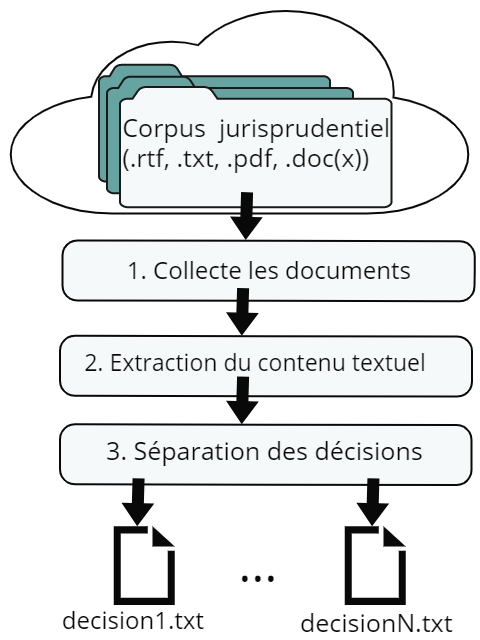
\includegraphics [width=0.45\textwidth]{structuration-preprocess.png}
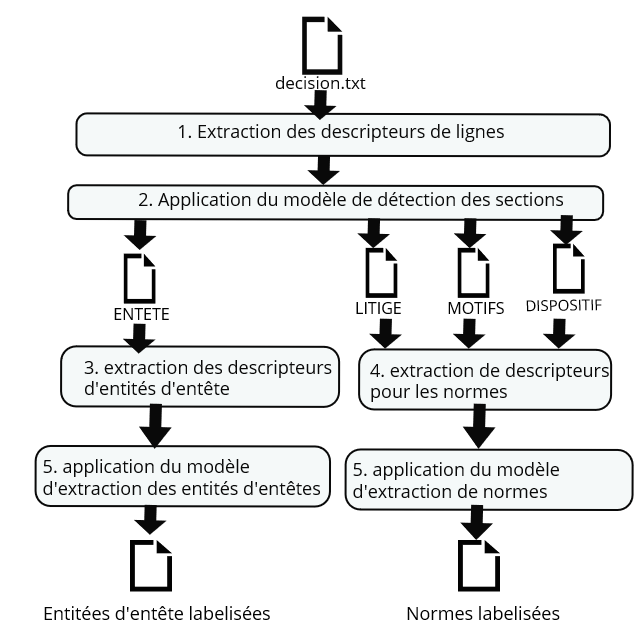
\includegraphics [width=0.45\textwidth]{structuration-pipeline-application.png}

{\scriptsize Après la collecte et le pretraitement des documents, l'étiqueteur de ligne est d'abord appliqué pour détecter les sections, puis les étiqueteurs d'entités peuvent être appliqués simultanement dans differentes sections.}
\caption{Application des modèles entrainés d'étiquetage de section et entités.}\label{p4_archAppli}
\end{figure}
Nous proposons de travailler uniquement avec le contenu textuel des documents. Ce contenu est extrait des documents téléchargés en eliminant les éléments inutiles, principalement des espaces vides. Ces éléments sont typiques des documents formatés (.rtf, .doc(x), .pdf). Ils ne fournissent pas une indication standard sur le début des sections. Le choix de ne pas exploiter le formatage des documents permet d'avoir à gérer un nombre plus faible de diversités entre les textes tout appliquant le même processus de traitement à tout document indépendament de sont format d'origine. Une simple architecture d'étiquetage de sections et d'entités juridiques a été conçu avec cet uniformisation des documents comme point d'entrée. Ainsi, les documents sont collectés pui prétraités suivant leur format d'origine (extraction du texte et séparation des décisions apparaissant dans le même document).  Ensuite, après le sectionnement des décisions, les entitées sont identifiées dans les différentes sections. Cette section décrit quelques aspects de conception à prendre en compte dans le but d'obtenir de bons résultats à partir d'un tel système.

\begin{figure}[!h]
%\sidecaption
\centering
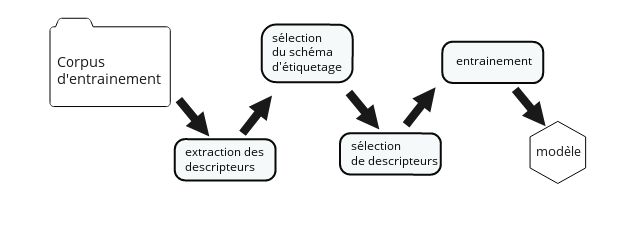
\includegraphics [width=\textwidth]{structuration-training.png}
\caption{Entrainement des modèles.}\label{fig:structuration:training}
\end{figure}


L'entrainement des modèles sur les exemples manuellement annotés est aussi décomposé en étapes. Nous proposons de sélectionner le schéma d'étiquetage, puis de sélectionner les sous-ensembles minimaux de caractéristiques manuellement définies, avant d'entrainer les modèles HMM et CRF (Figure \ref{fig:structuration:training}). La sélection de caractéristiques ne concerne pas l'implémentation en réseau de neuronnes du CRF.

\subsubsection{Descripteurs candidats}
\begin{table}[b]
    \centering
    \begin{tabular}{c|c}
         &  \\
         & 
    \end{tabular}
    \caption{Caractéristiques candidates pour l'identification de sections et d'entitées}
    \label{tab:my_label}
\end{table}

\subsection{Réseaux de neuronnes double-tache}
Découpage des 


\section{Expérimentations et discussions}
L'objectif de cette section est de discuter des différents aspects d'optimisation des performance des modèles CRF, HMM et BiLSTM-CRF, et de les comparer lorsqu'ils sont entrainés dans les conditions optimales déterminées empiriquement. Il est question de discuter l'effet des caractéristiques définies, de comparer des algorithmes de sélection de caractéristiques et des schémas d'étiquetage, de vérifier l'effet de l'augmentation des données d'entrainement sur la performance des modèles.

\label{sec:structuration:experimentations}
\subsection{Configuration des expérimentations}
\subsubsection{Annotation des données de référence}
Pour évaluer les méthodes de TAL, \citet{xiao2010corpuscreation} (\textcolor{red}{démontre l'importance...}) suggère de choisir un jeu de données échantillon suffisant en assurant l'équilibre dans la variété des données et la représentativité du langage. Cette en suivant cette recommendation que nous avons prétraité et annoté manuellement un ensemble de 503 documents à l'aide de la plateforme GATE Developer\footnote{https://gate.ac.uk/family/developer.html}. Cet outil permet de marquer avec le pointeur de la souris les passage à annoter; ce qui facilite l'annotation manuelle. Des balises XML sont rajoutées en arrières plan dans le document pour marquer les passages sélectionnés.

Chaque document comprend en moyenne 262,257 lignes et 3955,215 mots. La représentativité du corpus a été simulée en choisissant aléatoirement les décisions tout en faisant variés la ville et l'année. Les deux dernières colonnes du Tableau \ref{p4_relevantinfo} présente la distribution des entités labelisées dans le jeu de données. En se basant sur un sous-ensemble de 13 documents labelisés par 2 annotateurs différents, nous avons calculé des taux d'inter-agrément en utilisant la statistique Kapp de Cohen. Ces mesures d'inter-agrément ont été calculées au niveau des caractère parce que certains mots peuvent être coupés par des annotations incorrectes. (par ex. \textit{<juridiction>cour d'appe</juridiction>\underline{l}} vs. \textit{<juridiction>cour d'appe\underline{l}</juridiction>}), ou les annotateurs pourraient ne pas être d'accord un apostrophe doit être inclu ou pas (par ex. \textit{ \underline{l'}<norme>article 700} vs. \textit{ <norme>\underline{l'}article 700}). Les taux de Kappa de 0,705 et 0,974 ont été obtenu pour l'annotation des entités et des sections respectivement. D'après la catégorisation de \citet{viera2005kappa}, le niveau d'agrément observé est \textit{substentiel} pour les entités (0,61-0,80) et \textit{presque parfait} pour les sections (0,81 - 0,99).

\subsubsection{Protocole d'évaluation}
Nous avons utilisé la Précision, le rappel et la F1-mesure comme mesures d'évaluation car elles sont généralement utilisées comme référence en extraction d'information. Nous comparons deux niveaux de performances: i) à quel point le système est en mesure de bien labeliser chaque élément/mot d'entité (niveau-mot), et ii) à quel point le modèle labélise entièrement une entité (niveau-entité). Nous présentons aussi des performances au niveau micro i.e. les performances du classifieur en général sans distinction des classes. A tous les niveau d'évaluation, la F1-mesure se calcule à l'aide de la formule \ref{NER-f1-mesure}.  
\begin{equation}\label{NER-f1-mesure}
F1 = 2 \times \frac{Precision \times Rappel} {Precision + Rappel}
\end{equation}
%La précision et le rappel quant à eux se calculent suivant les formules
% \begin{equation}\label{NER-precision}
% Precision = \frac{TP}{}
% \end{equation}

\vspace{0.3cm}

\noindent \underline{\textbf{Evaluation au niveau atomique (\textit{token-level)}}}: Cette évaluation mésure la capacité d'un modèle à labeliser les éléments atomiques des entités à identifier. Les valeurs de précision and rappel sont calculés sur les données de test pour chaque label $l$ comme suit:
\[Precision_l = \frac{\text{nombre d'éléments correctement labelisés par le modèle avec } l} {\text{nombre d'éléments labelisés par le modèle avec } l}\]
\[Rappel_l = \frac{\text{nombre d'éléments correctement labelisés par le modèle avec } l} {\text{nombre d'éléments manuellement labelisés par le modèle avec } l}\]

\vspace{0.3cm}

\noindent \underline{\textbf{Evaluation au niveau entité (\textit{entity-level})}}: Cette évaluation mésure le taux d'entités parfaitement identifiées c'est-à-dire seulement ceux dont les éléments atomiques ont été tous correctement labélisés. Les valeurs de précision and rappel sont calculés sur les données de test pour chaque classe d'entité $e$ comme suit :
\[Precision_e = \frac{\text{nombre d'entités de type } e \text{ parfaitement détectées par le modèle}} {\text{nombre d'entités détectées et classifiées } e\text{ par le modèle}}\]
\[Rappel_e = \frac{\text{nombre d'entités de type } e \text{ parfaitement détectées par le modèle}} {\text{nombre d'entitées manuellement classifiées } e}\]

\vspace{0.3cm}

\noindent \underline{\textbf{Evaluation globale (\textit{overall-level})}}: L'évaluation globale donne les performances générales d'un modèle sans distinction des classes ou labels. Elle est réalisée aux deux niveaux décrits précédemment mais independamment du label d'élément ou du type d'entité :
\[Precision = \frac{\text{nombre d'entitées (resp. d'éléments) correctement detectées par le modèle}} {\text{nombre d'entitées (resp. d'éléments) detecteés par le modèle}}\]
\[Rappel = \frac{\text{nombre d'entitées (resp. d'éléments) correctement detectées par le modèle}} {\text{nombre d'entitées (resp. d'éléments)  manuellement annotatées}}\]

\subsubsection{Outils logiciels}
Nous avons utilisé les modèles HMM et CRF tels qu'implémentés dans la librairie Mallet \citep{McCallum2002Mallet}. Les modèles étudiés ont été entrainés par la méthode d'espérance maximale pour ceux basés sur le HMM, et par la méthode L-BFGS pour ceux basés sur le CRF. La \textit{tokenisation} des textes (découpage en élément atomique de type mots), ainsi que la lémmatisation et l'annotation des rôles grammaticaux (\textit{Part-of-Speech tagging}) ont été effetué à l'aide de la fonctionnalité d'annotation de texte français de TreeTagger \footnote{\url{http://www.cis.uni-muenchen.de/~schmid/tools/TreeTagger}}  \citep{schmid1994treetagger}. L'implémentation dans Mallet du LDA \citep{blei2003lda} a permis d'inférer 100 thèmes à partir d'un corpus lémmatisé d'environ 6k documents. Le tableau \ref{p4_topics} 
présente des mots représentatifs trouvés dans les premiers thèmes inférés. L'extraction des autres caractéristiques manuelles a été implémentée pour cette expérimentation. 

Les valeurs de précision, rappel, et F1-mesure ont été calculées à l'aide du script d'évaluation de la campagne CoNLL-2002 \footnote{\url{http://www.cnts.ua.ac.be/conll2002/ner/bin/conlleval.txt}}.

\begin{table}[!h]
\scriptsize
\begin{center}
\begin{tabular}{c|l}
Id thème & Mots représentatifs  \\ \hline
0	& 	préjudice  dommage  somme  subir  réparation  titre  faute  payer  intérêt  responsabilité  \\ \hline
1	& société  salarié  groupe  mirabeau  pouvoir  demande  article  licenciement  cour  titre    \\ \hline
2	& harcèlement  travail  salarié  moral  employeur  fait  attestation  faire  santé  agissements  \\ \hline
3	& vente  acte  prix  vendeur  acquéreur  notaire  condition  clause  vendre  immeuble  \\ \hline
4	& 		travail  poste  reclassement  employeur  médecin  licenciement  salarié  inaptitude  visite  \\ \hline
5	& 	monsieur  nîmes  avocat  appel  barreau  arrêt  madame  disposition  prononcer  président  \\ \hline
6	& 	mademoiselle  madame  non  mesure  décision  tutelle  surendettement  comparant   \\ \hline
7	& transport  marchandise  jeune  sed  éducateur  bateau  navire  transporteur  responsabilité  \\ \hline
8	&congé  salarié  conversion  emploi  plan  convention  employeur  sauvegarde  reclassement  \\ \hline
9	&marque  site  contrefaçon  sous  droit  auteur  joseph  produit  propriété  photographie  \\ \hline
10	&pierre  patrick  bordeaux  bruno  catherine  civil  article  corinne  cour  avocat\\ \hline
\end{tabular}
\end{center}
\caption{Mots représentatifs des 10 premiers thèmes sur les 100 inférés}\label{p4_topics}
\end{table}


\subsection{Sélection du schémas d'étiquetage}
Dans le but dévaluer comment la représentation de segment affecte les performances, nous avons implémenté quatre représentations (IO, IEO2, BIO2, BIEO).  Nos avons réalisé un simple découpage des données en deux ensembles: $25 \%$ pour l'entrainement et $75 \%$ pour les tests. Les performances reportées dans le Tableau \ref{fig:structuration:select-segm-repr} sont les performances globales sur la base de test. Seul l'élément (mot/ligne) est utilisé comme dscripteur. La durée d'entrainement est très longue, particulièrement pour la détection d'entité dans l'entête avec le CRF. Il semble évident que cette durée croit proportionnellement avec le nombre de labels possibles (BIEO exige beaucoup plus de temps, et IO exige le minimum de temps). Le schéma IOE semble être plus rapide à que BIO même s'ils ont le même nombre de labels. Nous remarquons aussi que les représentations complexes n'améliorent pas significativement les résultats par rapport au simple IO qui consomme pourtant le moins de temps.

\begin{table}[h]
\scriptsize
\caption{Comparaison des schémas d'étiquetage.}\label{fig:structuration:select-segm-repr}
\begin{center}
\begin{tabular}{p{0.9cm}|c|cccccccc}
\hline \noalign{\smallskip}
Tâche & Modèle & \multicolumn{3}{c}{Niveau atomique$^a$} & \multicolumn{3}{c}{Niveau entité$^a$} & \multirow{2}{*}{Durée$^b$} & Schéma \\
 & & Précision & Rappel & F1 &  Précision & Recall & F1 &  & \\ \hline %\noalign{\smallskip}\svhline\noalign{\smallskip}
\multirow{8}{*}{Sections}  & \multirow{4}{*}{CRF} & 91.75 & 91.75 & 91.75 & 64.49 & 56.55 & 60.26 &  4.685  & IO \\
&  & 88.95 & 88.95 & 88.95 & 48.12 & 38.26 & 42.63  & 11.877 & IEO2 \\
&  & 87.09 & 87.09 & 87.09 & 46.79 & 37.20 & 41.45 & 12.256 & BIO2 \\
 &  & 86.00 & 86.00 & 86.00 & 58.98 & 41.86 & 48.97  & 35.981 & BIEO \\ \cline{2-10}
& \multirow{4}{*}{HMM} & 32.64 & 32.64 & 32.64 & 22.16 & 18.91 & 20.41 & 6.564 & IO \\
&  & 32.92 & 32.92 & 32.92 & 17.73 & 16.09 & 16.87  &   7.827  & IEO2 \\
 &  & 32.39 & 32.39 & 32.39 & 31.93 & 26.65 & 29.05 & 8.391 & BIO2 \\
  &  & 33.06 & 33.06 & 33.06 & 32.47 & 27.53 & 29.80 & 8.7 & BIEO \\ \hline %
\multirow{8}{1.5cm}{Entités d'entête}  & \multirow{4}{*}{CRF} & 86.86 & 78.96 & 82.73 & 80.84 & 65.17 & 72.17  & 70.525 & IO \\
 &  & 87.77 & 79.65 & 83.51 & 82.46 & 65.19 & 72.82  & 228.751 & IEO2 \\
 &  & 87.41 & 78.14 & 82.51 & 81.66 & 66.80 & 73.49 & 230.865 & BIO2 \\
 &  & 87.72 & 79.55 & 83.44 & 84.38 & 68.35 & 75.53 &  475.249 & BIEO \\ \cline{2-10}
  & \multirow{4}{*}{HMM} & 79.12 & 67.75 & 73.00 & 61.48 & 35.05 & 44.64 & 6.345 & IO \\
  &  & 78.82 & 68.69 & 73.40 & 66.63 & 40.16 & 50.11& 8.298 & IEO2 \\ 
  &  & 80.68 & 67.48 & 73.49 & 70.37 & 45.32 & 55.14 & 7.908 & BIO2 \\
 &  & 80.05 & 69.01 & 74.12 & 74.73 & 50.77 & 60.46 & 9.973 & BIEO \\ \hline
\multirow{8}{*}{Normes}  & \multirow{4}{*}{CRF} & 95.60 & 92.96 & 94.26 & 88.06 & 83.50 & 85.72 & 28 & IO \\%
&  & 95.40 & 93.18 & 94.27 & 88.75 & 85.65 & 87.17 & 32.136 & IEO2 \\
 &  & 95.20 & 93.30 & 94.24 & 85.65 & 83.13 & 84.37 & 50.769 & BIO2 \\
  &  & 95.46 & 91.57 & 93.47 & 88.83 & 84.71 & 86.72 & 50.566 & BIEO \\ \cline{2-10}
  & \multirow{4}{*}{HMM} & 89.83 & 88.78 & 89.30 & 73.74 & 75.02 & 74.37 &  41.389 & IO \\%  
   &  & 88.20 & 89.23 & 88.71 & 78.01 & 81.27 & 79.61 & 44.086 & IEO2 \\
  &  & 89.25 & 87.83 & 88.53 & 73.89 & 76.63 & 75.24 & 46.634 & BIO2 \\
  &  & 87.39 & 88.10 & 87.74 & 77.76 & 82.35 & 79.99 & 45.52& BIEO \\ 
\noalign{\smallskip}\hline\noalign{\smallskip}
\end{tabular}
\end{center}

$^a$ Resultats sur une simple division du jeu de données en $25\%$ pour l'entrainement et  $75\%$ pour les tests (entrainement limité à 100 itérations au max)

$^b$ Durée d'entrainement en secondes avant l'arrêt de l'entrainement
\end{table}


\subsection{Sélection des descripteurs}
Pour comparer les méthodes BDS et SFFS, nous exploitons le schéma IO. Durant nos expérimentations, le SFFS a exécuté 185 entrainements pour le modèle CRF de d'identification des sections. La méthode BDS quant à elle à durée plus de 15h pour 600 sessions d'entrainement. Malgré la sauvegarde des scores F1 pour éviiter d'exécuter plusieurs fois l'entraimenent pour les mêmes sous-ensembles de descripteurs, le processus de sélection est resté toujours très long pour les deux algorithmes. Nous avons testé individuellement chacun des descripteurs candidat pour les modèles HMM. Les résultats sont repportés dans le Tableau \ref{fig:structuration:select-feats}.

Les descripteurs sélectionnés forment ds sous-ensembles inattendus étant donné que certains descripteurs spéciaux des voisins ont été choisis. Par exemple, dans le cas de la détection de section, la ligne suivante semble être beaucoup plus indicatrice que la première. Il est aussi intéressant de noter que les descripteurs basés sur notre observation apparaissent dans les sous-ensembles sélectionnés (par ex. isAfterIntervenant, isKEYWORD). Remarquons aussi que la longueur absolue des lignes (absLength)  joue un rôle majeur dans l'identification des sections vu qu'il a été sélectionné à la fois pour le CRF et le HMM (sélection BDS). Avec ses sous-ensembles sélectionnés de descripteurs, les modèles sont plus performants que lorsqu'ils ne doivent exploiter que l'élément ou tout l'ensemble des descripteurs candidats.  Cette amélioration des résultats reste insignifiante lorsqu'on considère la longue durée d'exécution des algorithmes. Ainsi, un algorithme meilleur et plus rapide devrait être utilisé à la place du SFFS et du BDS.

\begin{table}[!h]
\scriptsize
\caption{Effects of selected feature subsets on results.}\label{fig:structuration:select-feats}
\begin{center}
\begin{tabular}{l|c|ccc|ccc|c}
\hline\noalign{\smallskip}
Detection Task & Tagger & \multicolumn{3}{c}{niveau atomique$^a$} & \multicolumn{3}{c}{niveau entité$^a$}& Sous-ensemble \\
 & & Précision & Rappel & F1 &  Précision & Rappel & F1 & sélectionné\\
\noalign{\smallskip}\hline\noalign{\smallskip}
\multirow{7}{*}{Sections} 		& \multirow{4}{*}{CRF} & 99.31 & 99.31 & 99.31 & 90.28 & 90.68 & 90.48 & BDS$^{b1}$  \\
  				&  & 99.55 & 99.55 & \textbf{99.55} & 85.69 & 85.84 & 85.76 & \textbf{SFFS}$^{b2}$ \\
                &  & 99.36 & 99.36 & 99.36 & 88.16 & 88.39 & 88.27 & ALL* \\
                &  & 91.75 & 91.75 & 91.75 & 64.49 & 56.55 & 60.26 & token \\  \cline{2-9}
                 & \multirow{3}{*}{HMM} & 90.99 & 90.99 & \textbf{90.99}  & 4.18 & 3.63 & 3.89 & \textbf{absLength} \\ 
 & & 86.97 & 86.97 & 86.97 & 4.08 & 3.30 & 3.65 & relLength \\   
  &  & 37.59 & 37.59 & 37.59  & 18.81 & 18.81 & 18.81 & token \\ \hline
\multirow{7}{*}{Entités d'entête}	& \multirow{4}{*}{CRF} & 94.00 & 91.42 & 92.69 & 92.26 & 88.76 & 90.47 & BDS$^{c1}$  \\
				&  & 94.10 & 91.93 & \textbf{93.00} & 92.64 & 88.96 & 90.76 & \textbf{SFFS}$^{c2}$  \\ 
                &  & 94.20 & 91.86 & 93.02 & 93.05 & 89.59 & 91.28 & ALL \\
                &  & 86.86 & 78.96 & 82.73 & 80.84 & 65.17 & 72.17 & token \\ \cline{2-9}
                  &  \multirow{3}{*}{HMM}  & 76.90 & 80.41 & \textbf{78.61} & 62.66 & 52.16 & 56.93 &  \textbf{token} \\ 
  &    & 66.48 & 69.67 & 68.04 & 39.34 & 28.36 & 32.96 &  lemma\_W0 \\ 
  &    & 39.63 & 37.50 & 38.54 & 15.49 & 5.35 & 7.95 &  POS \\ \hline
\multirow{6}{*}{Normes} 			& \multirow{4}{*}{CRF} & 95.91 & 96.72 & 96.31 & 91.14 & 90.45 & 90.80 & \textbf{BDS}$^{d1}$ \\ 
				&  & 95.68 & 95.45 & 95.57 & 90.34 & 88.27 & 89.29 & SFFS$^{d2}$ \\ 
                &  & 95.07 & 96.69 & 95.87 & 90.87 & 90.64 & 90.76 & ALL \\
                &  & 95.60 & 92.96 & \textbf{94.26} & 88.06 & 83.50 & 85.72 & token \\ \cline{2-9}
                 &  \multirow{2}{*}{HMM} & 89.21 & 94.25 & 91.66 & 72.67 & 77.28 & 74.90 &  \textbf{token} \\ 
  &   & 90.31 & 92.81 & 91.54 & 69.24 & 69.46 & 69.35 &  lemma\_W0 \\ 
%  \noalign{\smallskip}\svhline\noalign{\smallskip}
%  & & token-level & entity-level & \\ \hline
\noalign{\smallskip}\hline\noalign{\smallskip}
\end{tabular}
\end{center}

$^a$ Resultats sur un simple découpage des données de $25\%$ pour l'entrainement,  $75\%$ pour le test avec 100 itérations d'entrainement au maximum  pour le CRF, et $80\%$ pour l'entrainement et $20\%$ pour le test avec 50 itérations au maximum pour l'entrainement du HMM

$^{b1}$ Selection par BDS pour les sections : [p0, n0, relNum, absLength, t0, t1, t2]

$^{b2}$ Selection par SFFS pour les sections: [n0, nRelLength, relNum, t0, t1, t2]

 $^{c1}$ Selection par BDS pour les entités d'entête:  [POSW1, isAfterAPPELANT, numInLine, w-2topic0, POSW2, isAfterINTERVENANT, isAfterINTIME, POSW-2, isLONELYINITIAL, token, lemma\_W0, lemmaW-2, isALLPUN, w-1, w1, w2, isALLCAP]

$^{c2}$ Selection par SFFS pour les  entités d'entête: [numInLine, w-2topic0, lemmaW-2, isAfterINTERVENANT, isAfterINTIME, w-1, w1, w2, isALLCAP, token]

$^{d1}$ Selection par BDS pour les normes: [POSW1, w-2topic0, isKEYWORD, lemmaW2, DIGIT-IN, token, lemmaW1, lemmaW-2, POS, isALLPUN, w-1, w2, PUN-IN, w-2]

$^{d2}$ Selection par SFFS pour les normes: [POSW1, lemmaW-2, w-1, DIGIT-IN]
\end{table}



\subsection{Evaluation détaillée pour chaque classe}
Nous discutons ici la capacité des modèles à identifier individuellement chaque type d'entité et de section. Les test ont été conduits avec tous les descripteurs pour les modèles CRF. Seuls \textit{absLength} et \textit{token} ont été utilisé comme descripteurs dans les modèles HMM pour l'identification des sections et des entités resp.. Le schéma d'étiquetage est IO. Le nombre d'itération maximal a été fixé à 500 pour assurer la convergence lors de l'entrainement même si les modèles HMM ne convergeaient jamais après 500 itérations. Les Tableaux \ref{tab:structuration:perf-detail-token} et \ref{tab:structuration:perf-detail-entity} présentent les résultats d'une 5-fold validation croisée au niveau des éléments et des entités, resp.. D'un point de vue général, les modèles HMM se comportent assez bien au niveau élément avec un seul descripteur, particulièrement pour l'identification des sections et des normes. Le modèle HMM est capable de labeliser les normes grâce à la mention des mêmes normes entre les décisions et la syntaxe presque standard que respectent les mentions (\verb=article [IDENTIFIANT] [TEXTE D'ORIGINE]=). Le modèle HMM n'est cependant pas efficace pour détecter entièrement les mots des entités d'où le faible score enregistré au niveau entité. Quant aux CRF, leurs résultats sont bons pour toutes les tâches et à tous les niveaux d'évaluation malgré certaines limites observées sur l'identification des mentions de parties.

\begin{table}[!h]
\centering
\scriptsize
\begin{subfigure}[t]{0.45\textwidth}
\centering
\begin{tabular}{|l|ccc|}
\hline
        & Precision  &  Recall   & F1 \\\hline
I-corps &   92.46 &  95.25 &  93.83 \\
I-dispositif &   53.44 &  48.46 &  50.83 \\
I-entete &   97.91 &  91.93 &  94.83 \\\hline
Overall &   90.63 &  90.63 &  90.63 \\\hline
 \noalign{\smallskip}\hline\noalign{\smallskip}
I-appelant &   34.46 &  16.87 &  22.65 \\
I-avocat &   85.17 &  98.75 &  91.46 \\
I-date  &   75.67 &  72.45 &  74.02 \\
I-fonction &   88.81 &  64.46 &  74.70 \\
I-formation &   79.38 &  94.38 &  86.23 \\
I-intervenant &   82.07 &  38.04 &  51.98 \\
I-intime &   50.40 &  68.09 &  57.93 \\
I-juge  &   73.40 &  88.73 &  80.34 \\
I-juridiction &   85.15 &  98.37 &  91.28 \\
I-rg    &   68.53 &  22.14 &  33.47 \\
I-ville &   91.50 &  82.41 &  86.72 \\\hline
Overall &   76.21 &  82.26 &  79.12 \\\hline
 \noalign{\smallskip}\hline\noalign{\smallskip}
I-norme &   88.23 &  93.70 &  90.89 \\\hline
\end{tabular}
\caption{Modèles HMM avec les descripteurs \textit{absLength} and \textit{token} pour l'identification resp. de section et d'entités et le schéma d'étiquetage IO.}\label{tab:structuration:perf-detail-token-hmm}
\end{subfigure} 
\hfill
\begin{subfigure}[t]{0.45\textwidth}
\centering
\begin{tabular}{|l|ccc|}
\hline
         & Precision &  Recall  & F1 \\\hline
I-corps &   99.57 &  99.69 &  99.63 \\
I-dispositif &   98.63 &  97.59 &  98.11 \\
I-entete &   99.51 &  99.55 &  99.53 \\\hline
Overall &   99.48 &  99.48 &  99.48 \\\hline
 \noalign{\smallskip}\hline\noalign{\smallskip}
I-appelant &   84.34 &  76.27 &  80.10 \\
I-avocat &   98.02 &  98.15 &  98.09 \\
I-date  &   98.00 &  96.60 &  97.30 \\
I-fonction &   95.23 &  95.13 &  95.18 \\
I-formation &   98.80 &  99.45 &  99.12 \\
I-intervenant &   83.38 &  68.26 &  75.07 \\
I-intime &   82.54 &  83.33 &  82.93 \\
I-juge  &   97.55 &  97.23 &  97.39 \\
I-juridiction &   98.91 &  99.69 &  99.30 \\
I-rg    &   97.81 &  97.44 &  97.62 \\
I-ville &   98.94 &  99.15 &  99.04 \\\hline
Overall &   95.13 &  94.51 &  94.82 \\\hline
 \noalign{\smallskip}\hline\noalign{\smallskip}
I-norme &   97.14 &  96.09 &  96.62 \\\hline
\end{tabular}
\caption{Modèles CRF avec tous les descripteurs et le schéma IO}\label{tab:structuration:perf-detail-token-crf}
\end{subfigure} 
\caption{Précision, Rappel, F1-mesures pour chaque type d'entité et section au niveau atomique.}\label{tab:structuration:perf-detail-token}
\end{table}

\begin{table}[!h]
\centering
\scriptsize
\begin{subfigure}[t]{0.45\textwidth}
\centering
\begin{tabular}{|l|ccc|}
\hline
        & Precision &  Recall  & F1 \\\hline
corps   &    0.99 &   0.99 &   0.99 \\
dispositif &   12.05 &   7.33 &   9.11 \\
entete  &   10.47 &  10.50 &  10.48 \\\hline
Overall &    7.22 &   6.27 &   6.71 \\\hline
 \noalign{\smallskip}\hline\noalign{\smallskip}
appelant &   17.84 &   5.60 &   8.52 \\
avocat  &   44.29 &  39.15 &  41.56 \\
date    &   66.87 &  62.15 &  64.43 \\
fonction &   89.84 &  64.13 &  74.84 \\
formation &   61.50 &  65.86 &  63.61 \\
intervenant &   14.29 &   4.00 &   6.25 \\
intime  &   30.28 &  27.47 &  28.80 \\
juge    &   73.54 &  83.21 &  78.07 \\
juridiction &   81.31 &  87.66 &  84.37 \\
rg      &   68.53 &  22.41 &  33.77 \\
ville   &   89.52 &  84.70 &  87.05 \\\hline
Overall &   64.59 &  54.56 &  59.15 \\\hline
 \noalign{\smallskip}\hline\noalign{\smallskip}
norme   &   71.94 &  78.45 &  75.05 \\\hline
\end{tabular}
\caption{Modèles HMM avec les descripteurs \textit{absLength} and \textit{token} pour l'identification resp. de section et d'entités et le schéma d'étiquetage IO.} \label{tab:structuration:perf-detail-entity-hmm}
\end{subfigure} 
\hfill
\begin{subfigure}[t]{0.45\textwidth}
\centering
\begin{tabular}{|l|ccc|}
\hline
         & Precision &  Recall  & F1 \\\hline
corps   &   89.57 &  90.10 &  89.83 \\
dispositif &   98.02 &  97.82 &  97.92 \\
entete  &   92.11 &  92.48 &  92.29 \\\hline
Overall &   93.22 &  93.47 &  93.34 \\\hline
 \noalign{\smallskip}\hline\noalign{\smallskip}
appelant &   84.05 &  77.29 &  80.53 \\
avocat  &   90.97 &  90.30 &  90.63 \\
date    &   97.96 &  96.60 &  97.27 \\
fonction &   96.89 &  96.94 &  96.92 \\
formation &   98.40 &  98.95 &  98.68 \\
intervenant &   62.50 &  40.00 &  48.78 \\
intime  &   79.31 &  78.93 &  79.12 \\
juge    &   96.58 &  96.35 &  96.47 \\
juridiction &   98.86 &  99.54 &  99.20 \\
rg      &   97.57 &  98.02 &  97.79 \\
ville   &   98.85 &  99.15 &  99.00 \\\hline
Overall &   93.77 &  92.93 &  93.35 \\\hline
 \noalign{\smallskip}\hline\noalign{\smallskip}
norme   &   92.66 &  91.38 &  92.01 \\\hline
\end{tabular}
\caption{Modèles CRF avec tous les descripteurs et le schéma IO}\label{tab:structuration:perf-detail-entity-crf}
\end{subfigure} 
\caption{Précision, Rappel, F1-mesures pour chaque type d'entité et section au niveau entité.}\label{tab:structuration:perf-detail-entity}
\end{table}


\subsection{Analyse des erreurs}
\subsubsection{Confusion de classes}
Certaines erreurs sont probablement dûe à la proximité des entités de types différents. D'après la matrice de confusion (Figure \ref{fig:structuration:matrices-confusions}), les \textit{intervenants} sont souvent classifiés comme \textit{intimé} ou \textit{avocat} probablement parce qu'il s'agit d'individus mentionnés les uns à la suite des autres dans l'entête (les \textit{intervenants} sont mentionnés juste après les \textit{avocats} des \textit{intimés}). Certaines mentions d'\textit{appelant} sont aussi classifiées comme \textit{intimés} dans plusieurs documents. La proximité crèe aussi des confusions entre des sections qui se suivent c'est-à-dire entre ENTETE et CORPS, et entre CORPS ET DISPOSITIF.  

\begin{figure}[h!]
    \centering
    %\includegraphics{}
    \textcolor{red}{Matrices de confusion}
    \caption{Matrices de confusion}
    \label{fig:structuration:matrices-confusions}
\end{figure}

\subsubsection{Redondance des mentions d'entitées}
Il est aussi intéressant de remarquer que certaines entitées sont repétées dans le document. Par exemple, les des parties sont mentionnées précédemment à une autre mention qui donne plus de détail sur eux. Certaines normes sont aussi citées de manière repétée et en alternant souvent les formes allongées et les formes longues. Malgré le fait que les mentions repétées ne sont pas identiques, de telles redondance aident à réduire le risque de manquer une entité. Cette aspect peut être exploité afin de combler l'imperfection des modèles.

\subsubsection{Découpage atomique}

\subsubsection{Impact de la quantité d'exemples annotées}
Certaines expérimentations ont été conduites pour évaluer comment les modèles s'améliorent lorsqu'on augmente le nombre de données d'entrainement. Pour cela, nous avons calculé les performances des modèles pour de différentes taille de la base d'entrainement. Les données ont été divisées en $75\%-25\%$ pour resp. l'entrainement et le test. Seules 20 fractions de l'ensembles d'entrainement ont été testées (de 5\% à 100\%). A chasue session entrainement-test, le même jeu de test a été utilisé pour les différentes fractions de l'ensemble d'entrainement. Les courbes d'apprentissage des modèles CRF et HMM sont représentées resp. sur les Figures \ref{fig:structuration:learning-curves-crf} et \ref{fig:structuration:learning-curves-hmm}. Il est évident que les scores F1 croissent avec plus de données d'entrainement pour les CRF et HMM, mais cette amélioration devient très faible au-delà de 60\% de données d'entrainement quelque soit la tâche. Il est possible que les exemples rajoutés à partir de là partagent la même structure qu'une majorité d'autres. Ainsi, cette étude doit être étendue à la sélection des exemples les plus utiles. \citet{raman2003exampleSelection} a demonstré les avantages des algorithmes de sélection d'exemples combinés à la sélection de caractéristique pour la classification. Les mêmes méthodes sont probablement applicables à l'étiquetage de séquence.

\begin{figure}[!htb]
\centering
\begin{subfigure}[t]{0.95\textwidth}
\centering
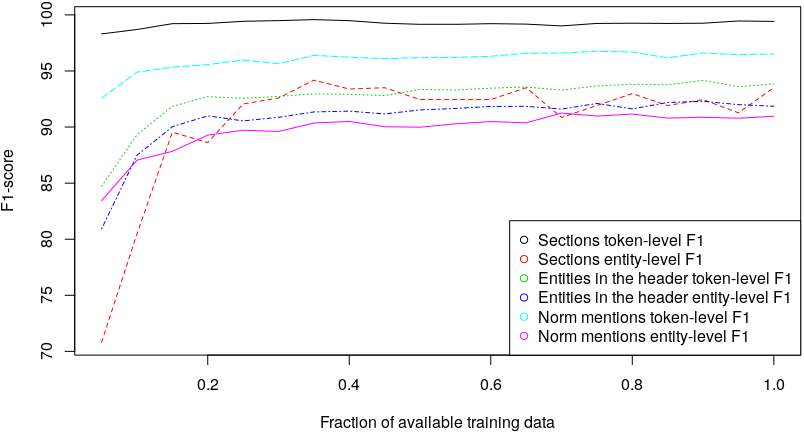
\includegraphics[width=0.95\textwidth]{lc-crf.png}
\caption{CRF} \label{fig:structuration:learning-curves-crf}
\end{subfigure} 

\begin{subfigure}[t]{0.95\textwidth}
\centering
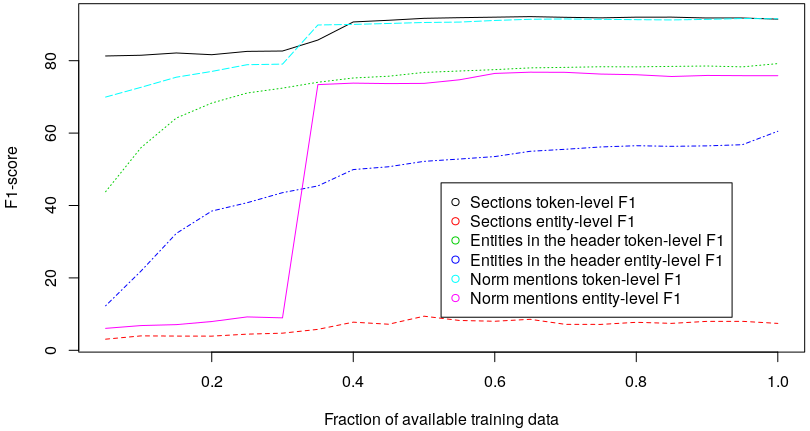
\includegraphics[width=0.95\textwidth]{lc-hmm.png}
\caption{HMM} \label{fig:structuration:learning-curves-hmm}
\end{subfigure}
\caption{Courbes d'apprentissages aux niveaux élément et entité} \label{fig:structuration:learning-curves}
\end{figure}

\section{Conclusion}
\label{sec:structuration:conclusion}
